\documentclass[11pt]{article} % type of the document
\usepackage[english]{babel} % language of all the auto generated text
\usepackage{lmodern} % use a high quality font
\usepackage{listings} % include code snippets
\usepackage{color} % use colors
\usepackage{textcomp} % additional symbols
\usepackage[hyphens]{url} % adds the \url command
\usepackage[hidelinks]{hyperref}
\usepackage{graphicx} % used for graphics stuff
\usepackage{subcaption} % allows adding subfigures
\usepackage{fancyhdr} % header and footer
\usepackage{todonotes} % \todo command
\usepackage{everypage} % run stuff on every page
\usepackage{pdfpages} % include pdf files as figures
\usepackage[noindentafter]{titlesec}
\usepackage{xspace} % add spaces after macros if necessary
\usepackage{amstext} % includes the \text command
\usepackage{booktabs} % table styling
\usepackage{lipsum} % lorem ipsum
\usepackage{enumitem}
\usepackage{float} % absolute positioning of floats
\usepackage{amsfonts} % additional fonts (used for \textbb
\usepackage{booktabs} % table styling
\usepackage{longtable} % repeat table header on each page
\usepackage{xspace} % used to correct spacing after abbreviations
\usepackage{amssymb,array}
\usepackage{enumitem}
\usepackage{geometry} % define the geometry of the page
\geometry{a4paper,left=25mm,right=25mm, top=28mm, bottom=28mm} 

\setcounter{tocdepth}{5} % define the depth of the table of contents
\setcounter{secnumdepth}{5} % define the depth of the section structure

% paragraphs look like subsubsubsections
\titleformat{\paragraph}[hang]{\bf}{\thetitle\quad}{0pt}{}
\titlespacing{\paragraph}{0pt}{1em}{0.5em} 

% subparagraphs look like paragraphs used to look
\titleformat{\subparagraph}[runin]{\bf}{}{0.5em}{}
\titlespacing{\subparagraph}{0pt}{1em}{1em}

\newcommand{\Ra}{\ensuremath{\Rightarrow}\xspace}
\newcommand{\ra}{\ensuremath{\rightarrow}\xspace}

\definecolor{dark-gray}{gray}{0.3}

\newcommand{\floatright}[1]{\hfill \textcolor{dark-gray}{#1}}

% adds a foot rule to every page
\AddEverypageHook
{
    \renewcommand{\footrulewidth}{0.4pt}
}

% define escape characters for latex commands in listings
\lstset{%
  escapeinside={(*}{*)},%
}

% define symbols for optional and non-optional properties
\newcommand{\nonoptional}{\ensuremath{{}^{\textbf{\circ}}}}
\newcommand{\nonoptionalif}{\ensuremath{{}^{\textbf{*}}}}

% define minipage in tabular
\newcommand{\cellwrap}[1]{\begin{minipage}[t]{1.0\columnwidth}#1\end{minipage}}

% define abbreviations properly
\newcommand*{\eg}{e.g.\@\xspace}
\newcommand*{\ie}{i.e.\@\xspace}

\newcommand{\pipe}{\ensuremath{|}\xspace}

% define colored text method
\newcommand{\coloredtext}[1]{\color[HTML]{#1}{\##1}}

\renewcommand{\thesubfigure}{\Alph{subfigure}}

%%%%%%%%%% DEFINE VARIABLES HERE %%%%%%%%%%%%%%%
\newcommand{\instanceStuff}{\texttt{instance-stuff}}


%%%%%%%%%% TIKZ DEFINITIONS %%%%%%%%%%%%


% style the header and footer
\pagestyle{fancy}
\renewcommand{\sectionmark}[1]{\markright{#1}}
\fancyfoot[R]{\thepage}
\fancyfoot[C]{}
\fancyhead[L]{Germinate 3}
\fancyhead[R]{\nouppercase{\rightmark}}

\hypersetup{
	pdfauthor={Sebastian Raubach},
	pdftitle={Germinate 3 User Guide},
	pdfinfo={Copyright={Copyright 2013-\the\year The James Hutton Institute. All rights reserved.}}
}

\makeatletter
\lst@CCPutMacro\lst@ProcessOther {"2D}{\lst@ttfamily{-{}}{-{}}}
\@empty\z@\@empty
\makeatother

% the document starts here
\begin{document}

% remove page numbers for title and TOC
\pagenumbering{gobble}
% title page is compiled by itself
\includepdf{title.pdf}

% add the table of contents
\tableofcontents

% Include the styling of the code snippets
%\include{theme-dark}
% code styling for java
\lstdefinestyle{Java}{
	backgroundcolor=\color[RGB]{240,240,240},
	tabsize=4,
	rulecolor=\color[RGB]{200,200,200},
    frame=tblr,
    framerule=0.1pt,
    framexleftmargin=0pt,
	language=java,
    basicstyle=\scriptsize\color[rgb]{0,0,0},
    upquote=true,
    aboveskip={0.5\baselineskip},
    columns=fullflexible,
    showstringspaces=false,
    extendedchars=true,
    breaklines=true,
    prebreak=,
    showtabs=false,
    showspaces=false,
    showstringspaces=false,
    identifierstyle=\ttfamily,
    keywordstyle=\color[RGB]{32,96,160},
    commentstyle=\color[RGB]{70,70,70},
    stringstyle=\color[RGB]{0,153,51},
    morekeywords={@Override,@RemoteServiceRelativePath,@PluralCount},
}

% code styling for javascript
\lstdefinestyle{JavaScript}{
	backgroundcolor=\color[RGB]{240,240,240},
	tabsize=4,
	rulecolor=\color[RGB]{200,200,200},
	frame=tblr,
	framerule=0.1pt,
	framexleftmargin=0pt,
	language=,
	basicstyle=\scriptsize\color[rgb]{0,0,0},
	upquote=true,
	aboveskip={0.5\baselineskip},
	columns=fullflexible,
	showstringspaces=false,
	extendedchars=true,
	breaklines=true,
	prebreak=,
	showtabs=false,
	showspaces=false,
	showstringspaces=false,
	identifierstyle=\ttfamily,
	keywordstyle=\color[RGB]{32,96,160},
	commentstyle=\color[RGB]{70,70,70},
	stringstyle=\color[RGB]{0,153,51},
	keywords={typeof, new, true, false, catch, function, return, null, catch, switch, var, if, in, while, do, else, case, break},
	morestring=[b]",
	morestring=[b]'
}



% code styling for HTML
\lstdefinestyle{HTML}{
	backgroundcolor=\color[RGB]{240,240,240},
	tabsize=4,
	rulecolor=\color[RGB]{200,200,200},
    frame=tblr,
    framerule=0.1pt,
    framexleftmargin=0pt,
	language=java,
    basicstyle=\scriptsize\color[rgb]{0,0,0},
    upquote=true,
    aboveskip={0.5\baselineskip},
    columns=fullflexible,
    showstringspaces=false,
    extendedchars=true,
    breaklines=true,
    prebreak=,
    showtabs=false,
    showspaces=false,
    showstringspaces=false,
    identifierstyle=\ttfamily,
    keywordstyle=\color[RGB]{32,96,160},
    commentstyle=\color[RGB]{70,70,70},
    stringstyle=\color[RGB]{0,153,51},
    morekeywords={},
}

% code styling for the .properties files
\lstdefinestyle{Properties}{
	backgroundcolor=\color[RGB]{240,240,240},
	tabsize=4,
	rulecolor=\color[RGB]{200,200,200},
    frame=tblr,
    framerule=0.1pt,
    framexleftmargin=0pt,
	language=,
    basicstyle=\scriptsize\color[rgb]{0,0,0},
    upquote=true,
    aboveskip={0.5\baselineskip},
    columns=fullflexible,
    showstringspaces=false,
    extendedchars=true,
    breaklines=true,
    prebreak=,
    showtabs=false,
    showspaces=false,
    showstringspaces=false,
    identifierstyle=\ttfamily,
    keywordstyle=\color[RGB]{32,96,160},
    commentstyle=\color[RGB]{70,70,70},
    stringstyle=\color[RGB]{0,153,51},
    morekeywords={Germinate,GerminateGatekeeper,Database,Username,Password,Server,Name,UsePort,Port,UseAuthentication,
    Debug,KeepTemporaryFileForHours,Template,VersionName,VersionLink,VersionImage,VersionNumber,Title,DatabaseName,
    TwitterLink,Copyright,Flapjack,Path,CreateProjectMain,AvailablePages,BaseSearchColumn,menuMyFanyPage,iSeeTrees,
    welcomeMessage,LogoMap,BaseTableExternalLink,BaseTableExternalLinkColumn,CollectingsiteTreemapColumn,CookieLifespanMinutes,
    AlleleFreq,MakeHistogram,CreateImage,BinData,Java,R,Gatekeeper,HighlightColor,Menu,GradientTop,GradientBottom,
    CategoricalColors,GradientColors,EmailAddress,ShowHomeOnLogin,BCrypt,Rounds,Registration,Enabled,Needs,Approval,GoogleAnalytics,TrackingId,
    CookieNotifier,UploadSizeLimitMB,Social,ShowFacebook,ShowTwitter,ShowGooglePlus,URL,Server,Logging,IsUnderMaintenance,
    ExternalDataFolder,HideIdColumns,AccessionDisplayColumn,IsReadOnly,Gallery,Images,Per,Page,UseToggleSwitches,Show,Search,Logo,Contains,Link,Show,Parallax,Banner,CustomMenu}
}

\lstdefinestyle{CSS}{
    backgroundcolor=\color[RGB]{240,240,240},
	tabsize=4,
	rulecolor=\color[RGB]{200,200,200},
    frame=tblr,
    framerule=0.1pt,
    framexleftmargin=0pt,
	language=,
    basicstyle=\scriptsize\color[rgb]{0,0,0},
    upquote=true,
    aboveskip={0.5\baselineskip},
    columns=fullflexible,
    showstringspaces=false,
    extendedchars=true,
    breaklines=true,
    prebreak=,
    showtabs=false,
    showspaces=false,
    showstringspaces=false,
    identifierstyle=\ttfamily,
    keywordstyle=\color[RGB]{32,96,160},
    commentstyle=\color[RGB]{70,70,70},
    stringstyle=\color[RGB]{0,153,51},
    morekeywords={accelerator,azimuth,background,background-attachment,
	    background-color,background-image,background-position,
	    background-position-x,background-position-y,background-repeat,
	    behavior,border,border-bottom,border-bottom-color,
	    border-bottom-style,border-bottom-width,border-collapse,
	    border-color,border-left,border-left-color,border-left-style,
	    border-left-width,border-right,border-right-color,
	    border-right-style,border-right-width,border-spacing,
	    border-style,border-top,border-top-color,border-top-style,
	    border-top-width,border-width,bottom,caption-side,clear,
	    clip,color,content,counter-increment,counter-reset,cue,
	    cue-after,cue-before,cursor,direction,display,elevation,
	    empty-cells,filter,float,font,font-family,font-size,
	    font-size-adjust,font-stretch,font-style,font-variant,
	    font-weight,height,ime-mode,include-source,
	    layer-background-color,layer-background-image,layout-flow,
	    layout-grid,layout-grid-char,layout-grid-char-spacing,
	    layout-grid-line,layout-grid-mode,layout-grid-type,left,
	    letter-spacing,line-break,line-height,list-style,
	    list-style-image,list-style-position,list-style-type,margin,
	    margin-bottom,margin-left,margin-right,margin-top,
	    marker-offset,marks,max-height,max-width,min-height,
	    min-width,-moz-binding,-moz-border-radius,
	    -moz-border-radius-topleft,-moz-border-radius-topright,
	    -moz-border-radius-bottomright,-moz-border-radius-bottomleft,
	    -moz-border-top-colors,-moz-border-right-colors,
	    -moz-border-bottom-colors,-moz-border-left-colors,-moz-opacity,
	    -moz-outline,-moz-outline-color,-moz-outline-style,
	    -moz-outline-width,-moz-user-focus,-moz-user-input,
	    -moz-user-modify,-moz-user-select,orphans,outline,
	    outline-color,outline-style,outline-width,overflow,
	    overflow-X,overflow-Y,padding,padding-bottom,padding-left,
	    padding-right,padding-top,page,page-break-after,
	    page-break-before,page-break-inside,pause,pause-after,
	    pause-before,pitch,pitch-range,play-during,position,quotes,
	    -replace,richness,right,ruby-align,ruby-overhang,
	    ruby-position,-set-link-source,size,speak,speak-header,
	    speak-numeral,speak-punctuation,speech-rate,stress,
	    scrollbar-arrow-color,scrollbar-base-color,
	    scrollbar-dark-shadow-color,scrollbar-face-color,
	    scrollbar-highlight-color,scrollbar-shadow-color,
	    scrollbar-3d-light-color,scrollbar-track-color,table-layout,
	    text-align,text-align-last,text-decoration,text-indent,
	    text-justify,text-overflow,text-shadow,text-transform,
	    text-autospace,text-kashida-space,text-underline-position,top,
	    unicode-bidi,-use-link-source,vertical-align,visibility,
	    voice-family,volume,white-space,widows,width,word-break,
	    word-spacing,word-wrap,writing-mode,z-index,zoom},
    morestring=[s]{:}{;},
    alsodigit={-},
    sensitive,
    morecomment=[s]{/*}{*/}
}

% code styling for the Eclipse .properties files
\lstdefinestyle{EclipseProperties}{
	backgroundcolor=\color[RGB]{240,240,240},
	tabsize=4,
	rulecolor=\color[RGB]{200,200,200},
    frame=tblr,
    framerule=0.1pt,
    framexleftmargin=0pt,
	language=,
    basicstyle=\scriptsize\color[rgb]{0,0,0},
    upquote=true,
    aboveskip={0.5\baselineskip},
    columns=fullflexible,
    showstringspaces=false,
    extendedchars=true,
    breaklines=true,
    prebreak=,
    showtabs=false,
    showspaces=false,
    showstringspaces=false,
    identifierstyle=\ttfamily,
    keywordstyle=\color[RGB]{32,96,160},
    commentstyle=\color[RGB]{70,70,70},
    stringstyle=\color[RGB]{0,153,51},
    morekeywords={project,name,root,instance,files,tomcat,manager,url,username,password}
}

% code styling for xml files
\lstdefinestyle{Xml}{
	backgroundcolor=\color[RGB]{240,240,240},
	tabsize=4,
	rulecolor=\color[RGB]{200,200,200},
    frame=tblr,
    framerule=0.1pt,
    framexleftmargin=0pt,
	language=xml,
    basicstyle=\scriptsize\color[rgb]{0,0,0},
    upquote=true,
    aboveskip={0.5\baselineskip},
    columns=fullflexible,
    showstringspaces=false,
    extendedchars=true,
    breaklines=true,
    prebreak=,
    showtabs=false,
    showspaces=false,
    showstringspaces=false,
    identifierstyle=\ttfamily,
    keywordstyle=\color[RGB]{32,96,160},
    commentstyle=\color[RGB]{70,70,70},
    stringstyle=\color[RGB]{0,153,51},
}

% code styling for the .properties files
\lstdefinestyle{Proxy}{
	backgroundcolor=\color[RGB]{240,240,240},
	tabsize=4,
	rulecolor=\color[RGB]{200,200,200},
	frame=tblr,
	framerule=0.1pt,
	framexleftmargin=0pt,
	language=,
	basicstyle=\scriptsize\ttfamily\color[rgb]{0,0,0},
	upquote=true,
	keepspaces=true
	aboveskip={0.5\baselineskip},
	columns=fullflexible,
	showstringspaces=false,
	extendedchars=true,
	breaklines=true,
	prebreak=,
	showtabs=false,
	showspaces=false,
	showstringspaces=false,
	identifierstyle=\ttfamily,
	keywordstyle=\color[RGB]{32,96,160},
	commentstyle=\color[RGB]{70,70,70},
	stringstyle=\color[RGB]{0,153,51}
}

% start page numbering from here
\setcounter{page}{1}
\pagenumbering{arabic}

% include all the content files (without file extension)
% start page numbering from here
\setcounter{page}{1}
\pagenumbering{arabic}

\section{Introduction}
Germinate 3 is a generic platform for the storage and dissemination of multiple data types associated with genetic resource collections. Examples of the types of data that Germinate 3 currently supports are passport, phenotypic, field trial, pedigree, genetic and geographic location data. Our aim is to keep Germinate as flexible as possible and we will add support for additional data types over time.

Germinate not only acts as storage for experimental data but offers a user-friendly interface into the data and acts as a backend for analysis tools such as Helium for pedigree visualization, our graphical genotyping application Flapjack \cite{Flapjack} and CurlyWhirly for the simple display of xyz coordinate data such as PCO and PCA. All these tools are available from \url{https://ics.hutton.ac.uk}. We have also prioritised the development of tools to allow users to export data in a variety of formats for analysis in external applications such as R.

Germinate 3 builds on the existing Germinate 2 platform an adds additional tools, functionality and introduces a much more simple installation process over its predecessor. These changes also allow us to deploy Germinate both within server and desktop environments which was difficult with Germinate 2. We have also removed the limitation of requiring Linux, Germinate 3 is now compatible with any environments that have Apache Tomcat. Germinate 3 takes the Germinate platform away from its Perl roots and has been completely rewritten using the Google Web Toolkit (GWT) from Google. The underlying database is as it was and while we recommend using MySQL should be compatible with a number of relational database management systems with minor changes. 

The move from Perl to Java and GWT has allowed us to introduce a number of new features. Examples include full internationalization and localization support which allows us to offer Germinate in multiple languages if suitable translations exit as well as offering a more advanced and
responsive web-interface and user access control.

We hope that you find Germinate 3 useful and our vision is that Germinate forms platform on to which additional tools can be added over time. The common platform means that any additional functionality can be rolled out to all other Germinate installations which makes it both a flexible and continually evolving platform to help meet the needs of the genetic resources community.
 
If you encounter any problems, have ideas for features that would be useful to include in Germinate or just want to chat about the system then we would love to hear from you and we can be contacted in a number of ways. By email on \href{mailto:germinate@hutton.ac.uk}{\nolinkurl{germinate@hutton.ac.uk}}, or you can write to us at: \\
\\
Germinate,\\ 
Information \& Computational Sciences, \\
The James Hutton Institute, \\
Invergowrie, \\
Dundee, \\
DD2 5DA, UK. \\

\noindent
We also have a website (\url{https://ics.hutton.ac.uk/get-germinate}) that we keep up to date with current developments of Germinate and all our other analysis and visualization tools and you can follow us on Twitter \href{https://twitter.com/cropgeeks}{\nolinkurl{@cropgeeks}}.
\section{Overview}
In this section, we will explain the overall structure of {\germinate} along with an overview of the various data types that {\germinate} supports.

\subsection{Authentication}
{\germinate} can be used with or without user authentication. If the administrator of {\germinate} decided to enable authentication, you will be asked to log in using a username and password. Figure \ref{fig:overview:login} shows the login page of {\germinate}. If you already have a user account, simply enter the username and password into the provided text boxes.

If you do not have a user account, click on the link below the login button to create an account. You may get asked to agree to a license agreement before being able to create an account.

To modify your user account, you can log in to {\gatekeeper}, which is {\germinate}'s user authentication portal. It can be accessed from the help popup on the login page.

\begin{figure}
	\centering
	\includegraphics[width=0.85\linewidth]{img/overview/login.png}
	\caption{Depending on the configuration of {\germinate}, you may be asked to log in.}
	\label{fig:overview:login}
\end{figure}

\subsection{Page layout}
Figure \ref{fig:overview:home} shows the main layout of the {\germinate} web interface. The main menu of {\germinate} is positioned to the left (Figure \ref{fig:overview:home}A). It is used to navigate between pages. Submenus can be expanded by simply clicking on the items showing the caret symbol. The menu is explained in more detail in Section \ref{sec:features:menu}. The overall search feature, shown in Figure \ref{fig:overview:home}B, allows you to run a full-text search across the whole database. The results will be grouped into topical categories. See Section \ref{sec:features:search} for more details. The interface has a banner along the top containing the {\germinate} logo and a few dropdown menu items in the top right corner (\cf Figure \ref{fig:overview:home}C). These items include the language selector which will be covered in Section \ref{sec:features:language-selector}, social media buttons, the marked item lists covered in Section \ref{sec:features:marked-items}, a user menu with specific functions based on your type of account, a "contact us" button and, finally, a help button that can be clicked to get more information about the current page (\cf Section \ref{sec:features:help}). An overview of the number of database items for certain types is shown in Figure \ref{fig:overview:home}D. Recent news about both the {\germinate} interface and the contained data are available in the news section shown in Figure \ref{fig:overview:home}E. Finally, a section about other projects that are related to the project you are currently looking at are available in Figure \ref{fig:overview:home}F.

\begin{figure}
	\centering
	\includegraphics[width=0.85\linewidth]{img/overview/home.png}
	\caption{The home page of {\germinate} is the first page you will see. (A) The main menu of {\germinate} used to navigate the page. (B) The search box used for free-text searches of the database. (C) Language selector, social media buttons, marked item lists, user menu and the help button. (D) An overview of number of data objects that are stored in {\germinate}. (E) Latest news about this instance of {\germinate} and the contained data. (F) Other projects that have a relation to the current project.}
	\label{fig:overview:home}
\end{figure}
\section{Features}
In this section, we will highlight the main features of {\germinate}. This section will expand as we add new features.

\subsection{Internationalization and Localization}
\label{sec:features_i18n}
{\germinate} fully supports internationalization for an unlimited number of languages. Every text that you can see on the web interface can be localized. The language used on start-up is chosen based on the browser settings, but the user can easily switch to a different language by selecting it from the combo box at the bottom of the page. Have a look at Section \ref{sec:example_i18n} for usage details.

\subsection{News}
The {\germinate} web interface contains a place holder to show the latest news of the project. On the database side, these news are stored in two tables and can be updated at any time. The web interface will check the availability of news and show the three latest entries at the bottom of the page. Changes on the database side will immediately be visible on the website.

\subsection{Available pages}
\label{sec:pages}
This section gives an overview of all the pages that are available for {\germinate}. Based on your requirements and the data that is available, you can decide which pages should actually be available on the web interface and hide all others. The set of available pages can be changed dynamically without having to re-deploy the application. This gives you the freedom to customize your {\germinate} experience just as you please.

\subsubsection{About {\germinate}}
\begin{description}
	\item[Content]\hfill\\The about page of {\germinate} shows information about {\germinate} itself. This includes information about the developers and contact details.
	\item[Page name]\hfill\\\texttt{about-germinate}
	\item[Used data]\hfill\\None
\end{description}

\subsubsection{About Project}
\begin{description}
	\item[Content]\hfill\\This page shows information about the project itself.
	\item[Page name]\hfill\\\texttt{about-project}
	\item[Used data]\hfill\\None
	\item[Customization] You can change the content of this page by providing HTML to the \texttt{page.\allowbreak about.\allowbreak project.\allowbreak text} property.
\end{description}

\subsubsection{Accessions Overview}
\begin{description}
	\item[Content]\hfill\\The overview page shows all the accessions contained in the {\germinate} database in a filterable table. The user can sort, filter and mark items. Below the table, there are tools to download accessions, their attributes and pedigree data to flat files.
	\item[Page name]\hfill\\\texttt{accession-overview}
	\item[Used data]\hfill\\biologicalstatus, collectingsources, countries, germinatebase, institutions, locations, locationtypes, mlsstatus, pedigreedefinitions, pedigreedescriptions, pedigreenotations, pedigrees, storage, storagedata, subtaxa, synonyms, synonymtypes, taxonomies 
\end{description}

\subsubsection{Accessions for Collecting Site}
\begin{description}
	\item[Content] This page shows all accessions that have been collected at the given collecting site. It also allows the user to download the data in .kml format for Google Earth.
	\item[Page name]\hfill\\\texttt{accessions-for-collsite}
	\item[Used data]\hfill\\germinatebase, locations, locationtypes, countries
	\item[URL parameter]\hfill\\\texttt{collectingsiteId} The id of the collecting site.
\end{description}

\subsubsection{Acknowledgements}
\begin{description}
	\item[Content]\hfill\\This page can be used to acknowledge collaborators, etc.
	\item[Page name]\hfill\\\texttt{acknowledgements}
	\item[Used data]\hfill\\None
	\item[Customization] You can change the content of this page by providing HTML to the \texttt{page.\allowbreak acknowledgements.\allowbreak text} property.
\end{description}

\subsubsection{Administrator Configuration}
\begin{description}
	\item[Content]\hfill\\This page allows page administrators to make modifications to the way {\germinate} operates and looks. Regular users cannot see this page.
	\item[Page name]\hfill\\\texttt{admin-config}
	\item[Used data]\hfill\\None
\end{description}

\subsubsection{Allele Frequency Datasets}
\begin{description}
	\item[Content]\hfill\\All available allele frequency datasets are shown on this page. The user will be able to select which datasets to export.
	\item[Page name]\hfill\\\texttt{allele-freq-dataset}
	\item[Used data]\hfill\\allelefrequencydata, datasets, datasetstates, datasetpermissions, germinatebase, experiments, experimenttypes
\end{description}

\subsubsection{Allele Frequency Export}
\begin{description}
	\item[Content]\hfill\\On this page, the user is able to select which data they want to export from the selected dataset.
	\item[Page name]\hfill\\\texttt{allele-freq-export}
	\item[Used data]\hfill\\allelefrequencydata, datasets, datasetstates, datasetpermissions, germinatebase, experiments, experimenttypes, groupmembers, groups, maps, mapdefinitions, mapfeaturetypes, markers, markertypes
	\item[URL parameter]\hfill\\\texttt{allelefreqDatasetIds} The id of the allele frequency dataset. Single selection only.
\end{description}

\subsubsection{Allele Frequency Results}
\begin{description}
	\item[Content]\hfill\\On this page, the user can select the data binning scheme they want to apply to the allele frequency data. The final output files are shown on this page as well.
	\item[Page name]\hfill\\\texttt{allele-freq-results}
	\item[Used data]\hfill\\allelefrequencydata, datasets, datasetstates, datasetpermissions, germinatebase, experiments, experimenttypes, groupmembers, groups, grouptypes, maps, mapdefinitions, mapfeaturetypes, markers, markertypes
\end{description}

\subsubsection{Climate Data}
\begin{description}
	\item[Content]\hfill\\The climate data page shows detailed information about climate information. The data is visualized in charts and a color-coded table. In addition, climate data map overlays are shown on a map.
	\item[Page name]\hfill\\\texttt{climate-data}
	\item[Used data]\hfill\\climatedata, climateoverlays, climates, countries, datasets, datasetpermissions, datasetstates, experiments, experimenttypes, germinatebase, groupmembers, groups, grouptypes, locations, locationtypes, units
\end{description}

\subsubsection{Climate Datasets}
\begin{description}
	\item[Content]\hfill\\All available climate datasets are shown on this page. The user will be able to select which datasets to export.
	\item[Page name]\hfill\\\texttt{climate-dataset}
	\item[Used data]\hfill\\climatedata, climates, datasets, datasetstates, datasetpermissions, germinatebase, experiments, experimenttypes
\end{description}

\subsubsection{Chemical Compounds}
\begin{description}
	\item[Content]\hfill\\This page shows a table with all the chemical compounds.
	\item[Page name]\hfill\\\texttt{compound-details}
	\item[Used data]\hfill\\analysismethod, compounddata, compounds, datasets, germinatebase, units
\end{description}

\subsubsection{Chemical Compound Details}
\begin{description}
	\item[Content]\hfill\\The chemical compound details page shows information about a specific compound. This includes the compound data values across all accessions and visible datasets as well as that same data in the form of a chart. If images and external links are associated with a compound, these will be shown as well.
	\item[Page name]\hfill\\\texttt{compound-details}
	\item[Used data]\hfill\\analysismethod, compounddata, compounds, datasets, germinatebase, synonyms, synonymtypes, units
	\item[URL parameter]\hfill\\\texttt{compoundId} The id of the chemical compound.
\end{description}

\subsubsection{Chemical Compound Datasets}
\begin{description}
	\item[Content]\hfill\\All available chemical compound datasets are shown on this page. The user will be able to select which datasets to export.
	\item[Page name]\hfill\\\texttt{compound-dataset}
	\item[Used data]\hfill\\compounddata, compounds, datasets, datasetstates, datasetpermissions, germinatebase, experiments, experimenttypes
\end{description}

\subsubsection{Chemical Compound Data}
\begin{description}
	\item[Content]\hfill\\This page offers various different visualizations for the chemical compound data of the selected datasets. The data can also be downloaded into flat files.
	\item[Page name]\hfill\\\texttt{compound-data}
	\item[Used data]\hfill\\analysismethod, compounddata, compounds, datasets, germinatebase, synonyms, synonymtypes, units
	\item[URL parameter]\hfill\\\texttt{compoundDatasetIds} The ids of the chemical compound dataset.
\end{description}

\subsubsection{Cookie}
\begin{description}
	\item[Content]\hfill\\EU law requires us to provide information about the cookies that {\germinate} uses and what we use this information for. Detailed information about our usage of cookies is available on this page.
	\item[Page name]\hfill\\\texttt{cookie}
	\item[Used data]\hfill\\None
\end{description}

\subsubsection{Data Statistics}
\begin{description}
	\item[Content]\hfill\\The data statistics page visualizes aggregated information about the data contained in {\germinate}.
	\item[Page name]\hfill\\\texttt{data-stats}
	\item[Used data]\hfill\\Everything
\end{description}

\subsubsection{Dataset Overview}
\begin{description}
	\item[Content]\hfill\\This page shows all the datasets within {\germinate} independent of their type in one table.
	\item[Page name]\hfill\\\texttt{dataset-overview}
	\item[Used data]\hfill\\allelefrequencydata, climatedata, climates, compounddata, compounds, datasets, datasetstates, datasetpermissions, germinatebase, experiments, experimenttypes, phenotypedata, phenotypes, units
\end{description}

\subsubsection{Experiment Details}
\begin{description}
	\item[Content]\hfill\\The experiment details page shows all the datasets contained in a single experiment.
	\item[Page name]\hfill\\\texttt{experiment-details}
	\item[Used data]\hfill\\datasets, datasetpermissions, datasetstates, experiments, experimenttypes
	\item[URL parameter]\hfill\\experimentId The id of the experiment.
\end{description}

\subsubsection{Genotype Datasets}
\begin{description}
	\item[Content]\hfill\\All available genotype datasets are shown on this page. The user will be able to select which datasets to export.
	\item[Page name]\hfill\\\texttt{genotype-dataset}
	\item[Used data]\hfill\\datasets, datasetstates, datasetpermissions, germinatebase, experiments, experimenttypes
\end{description}

\subsubsection{Genotype Export}
\begin{description}
	\item[Content]\hfill\\On this page, the user is able to select which data they want to export from the selected dataset.
	\item[Page name]\hfill\\\texttt{genotype-export}
	\item[Used data]\hfill\\datasets, datasetstates, datasetpermissions, germinatebase, experiments, experimenttypes, groupmembers, groups, maps, mapdefinitions, mapfeaturetypes, markers, markertypes
	\item[URL parameter]\hfill\\\texttt{genotypeDatasetIds} The id of the genotype dataset. Single selection only.
\end{description}

\subsubsection{Geographic Search}
\begin{description}
	\item[Content]\hfill\\The geographic search page allows the user to search for both accessions and locations based on a given query point or polygon.
	\item[Page name]\hfill\\\texttt{geographic-search}
	\item[Used data]\hfill\\countries, germinatebase, locations, locationtypes
\end{description}

\subsubsection{Group Preview}
\begin{description}
	\item[Content]\hfill\\ {\germinate} offers the functionality to define groups of accessions via an API and a dedicated page. Tools like CurlyWhirly can upload a file containing the identifier of accessions and {\germinate} will display a preview of these items in a table. Once the user is happy with the selection, they can create a new group based on the selection.
	\item[Page name]\hfill\\\texttt{group-preview}
	\item[Used data]\hfill\\germinatebase, groupmembers, groups, grouptypes
\end{description}

\subsubsection{Groups}
\begin{description}
	\item[Content]\hfill\\The groups page shows an overview of all the accession, marker and location groups that are defined in {\germinate}. Depending on the permissions, the user can create new groups, delete old groups and modify the members of a group.
	\item[Page name]\hfill\\\texttt{groups}
	\item[Used data]\hfill\\countries, germinatebase, groupmembers, groups, grouptypes, locations, locationtypes, markers, markertypes
	\item[URL parameter]\hfill\\\texttt{groupId} The id of the group.
\end{description}

\subsubsection{Image Gallery}
\begin{description}
	\item[Content]\hfill\\This page shows all the images that are defined grouped by type. By clicking on the button below each image the user will be able to navigate to the corresponding details page.
	\item[Page name]\hfil\\\texttt{image-gallery}
	\item[Used data]\hfill\\compounds, germinatebase, images, imagetypes
	\item[URL parameter]\hfill\\\texttt{latitude}, \texttt{longitude} The location of the point query.
\end{description}

\subsubsection{Locations}
\begin{description}
	\item[Content]\hfill\\The locations page shows information about the location data. The locations are displayed on maps as well as visualized in different ways.
	\item[Page name]\hfill\\\texttt{locations}
	\item[Used data]\hfill\\countries, germinatebase, locations, locationtypes
\end{description}

\subsubsection{Home}
\begin{description}
	\item[Content]\hfill\\The home page of {\germinate}. It shows aggregated statistics about accessions, groups, locations and markers.
	\item[Page name]\hfill\\\texttt{home}
	\item[Used data]\hfill\\countries, germinatebase, groupmembers, groups, grouptypes, locations, locationtypes, markers, markertypes
\end{description}

\subsubsection{Institutions}
\begin{description}
	\item[Content]\hfill\\This page shows all the institutions associated with accessions held in {\germinate}.
	\item[Page name]\hfill\\\texttt{institutions}
	\item[Used data]\hfill\\countries, germinatebsae, institutions, locations, locationtypes
\end{description}

\subsubsection{Maps}
\begin{description}
	\item[Content]\hfill\\The maps page shows an overview of all the maps. Selecting one of them will display a table of all the markers on this map along with their position on the chromosome.
	\item[Page name]\hfill\\\texttt{maps}
	\item[Used data]\hfill\\mapdefinitions, mapfeaturetypes, maps, markers, markertypes
	\item[URL parameter]\hfill\\\texttt{mapId} The id of a map. This will expand the details of this map.
\end{description}

\subsubsection{Marked Items}
\begin{description}
	\item[Content]\hfill\\Marked item lists are a way of keeping track of items of interest. These items can be any accessions, markers or locations that the user is interested in. The marked items page shows all the items a user has marked so far. There are options to download the data or to create a group from the list if the user has sufficient permissions.
	\item[Page name]\hfill\\\texttt{marked-items}
	\item[Used data]\hfill\\germinatebase, groupmembers, groups, grouptypes, markers, markertypes, locations, locationtypes
\end{description}

\subsubsection{Marker Details}
\begin{description}
	\item[Content]\hfill\\This page displays information about a single marker. It shows which datasets the marker is part of as well as which maps it is on. Additionally, a list of all known synonyms is shown.
	\item[Page name]\hfill\\\texttt{marker-details}
	\item[Used data]\hfill\\mapdefinitions, mapfeaturetypes, maps, markers, markertypes, synonyms, synonymtypes
	\item[URL parameter]\hfill\\\texttt{markerId} The id of the marker.
\end{description}

\subsubsection{Mega Environments}
\todo{TODO}

\subsubsection{News}
\begin{description}
	\item[Content]\hfill\\This page shows news about {\germinate} and the contained data. The news items are sorted by creation date, so the latest one is shown first.
	\item[Page name]\hfill\\\texttt{news}
	\item[Used data]\hfill\\news, newstypes
\end{description}


\subsection{User registration}
\label{sec:registration}

{\germinate} can be used with and without authentication. This means that you can decide if you want to restrict access to your {\germinate} instance to registered users. If you decide to do so, you'll need people to be able to register. The registration form of {\germinate} (Figure \ref{fig:user_registration_registration}) provides a concise and easy way to register. If you choose to use a disclaimer that potential new users have to accept, this will appear before the form is visible. Once the user completes the form, they will either get access right away or you need to approve the new users manually. This is based on the setting of the property \texttt{Gatekeeper.Registration.Needs.Approval} (see Section \ref{sec:config-properties} for help). If you choose to use the approval approach, you'll see the screen shown in Figure \ref{fig:user_registration_approval} after selecting "Approve users" in Gatekeeper. The user will be notified with your decision.

The registration agreement text the user has to agree to before signing up for your instance of {\germinate} is stored in the properties \texttt{page.\allowbreak registration.\allowbreak disclaimer.\allowbreak short.\allowbreak html} and \texttt{page.\allowbreak registration.\allowbreak disclaimer.\allowbreak long.\allowbreak html} in the \texttt{Text.properties} file. Translations of this text need to be placed in the appropriate internationalized version of this file.

\begin{figure}
    \centering
    \begin{subfigure}[b]{0.375\textwidth}
        \centering
        \includegraphics[width=1.0\textwidth]{img/features/registration.png}
        \caption{Registration form on the {\germinate} site}
        \label{fig:user_registration_registration}
    \end{subfigure}
    \hspace*{0.5cm}
    \begin{subfigure}[b]{0.575\textwidth}
        \centering
        \includegraphics[width=1.0\textwidth]{img/features/registration-approve.png}
        \caption{Approval page on the Gatekeeper page}
        \label{fig:user_registration_approval}
    \end{subfigure}
    \caption{User registration}
    \label{fig:user_registration}
\end{figure}

\subsection{Dataset licenses}
Sometimes it is required for individual datasets to be protected behind a license the user has to agree to before using the data. To accommodate this, we have introduced dataset licenses. Licenses are stored in the \texttt{licenses} table. The actual license content is stored in \texttt{licensedata} and linked to a \texttt{locale} so that you can have translations of your license content.

We keep track of which user accepted which license so that they are only prompted to accept new licenses. Make sure to remove associated \texttt{licenselogs} entries if you change the actual content of a license, because the user may originally have agreed to a different wording.

\subsection{Security}
\label{sec:example_security}
As already mentioned earlier, {\germinate} is equipped with a secure login system\footnote{{\germinate} is only as secure as the connection between client and server. Use a secure connection (TLS/SSL) to prevent password snooping.}. This feature is completely optional, but it allows you to protect your data from any unauthorized access. In this section, we will explain how the security system works and we will show what is necessary to use it properly.

\begin{figure}[h]
    \centering
    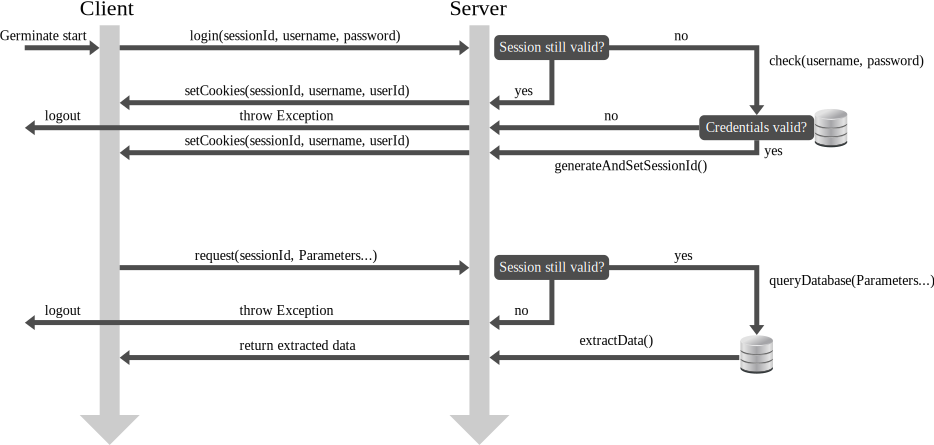
\includegraphics[scale=0.5]{img/examples/authentication.pdf}
    \caption{Authentication procedure of {\germinate}}
    \label{fig:authentication}
\end{figure}

Figure \ref{fig:authentication} shows the authentication process of {\germinate}. The figure contains two major parts. The upper part visualizes the login process, which is initialized by the user entering his/her credentials. These are sent to the server alongside any session id that is still stored in the client from previous sessions. The server will then check the session id that is received. If the id is still valid, the server will store the session id and return it to the client, which, in turn, will create a cookie containing this id.

If the session id is invalid, the server will check if the username password combination is genuine. This is done by encrypting the password and checking it against the entry in the database. If this check fails, the user will be logged out. Otherwise, the server will create a new session id, store it in the HTTP session and return it to the client, which will create a new cookie using this id. The login process is now complete and both the server (via HTTP session) and the client (via cookie) know the current session id.

For each new request that is made from the client, it will need to send the session id as the payload, \ie each remote procedure call (RPC) has to request the session id as a parameter to ensure the security of the communication. As a consequence if this, the server will receive the session id three times per request, namely via the HTTP session, via the cookie and via the payload. If all of these ids match up, the server can fulfil the client's request and return the data. However, if it fails, the user will be logged out.

As a final remark: Even if you currently do not want to enable the security feature, you should still write your code in a way that ensures it will work properly even when the security feature is enabled. Otherwise you might end up with a security leak.
\section{Data Types}
The following section will describe each data type that Germinate can handle in more detail. We will describe both the web interface that is used to display this data as well as what the export formats for each of the types are.

\subsection{Passport Data}

\subsubsection{Multi-Crop Passport Descriptors}
The Multi-Crop Passport Descriptors (MCPD) \cite{mcpd} is a widely used international standard to facilitate germplasm passport information exchange defined by the FAO. Germinate is fully MCPD V.2.1 compatible. The MCPD standard is used by many genebanks and genetic resources tools and utilities.

\subsection{Genotypic Data}
When we talk about genotypic data in the context of Germinate, we are referring to Single Nucleotide Polymorphic (SNP) or Simple sequence repeat (SSR) data. The data export process is shown in Figure \ref{fig:features:group-subselection}. After selecting the dataset you want to export, you can decide which accessions and markers should be included in the output. Data can be exported against different maps (cf. Section \ref{sec:features:genotypic-maps}), e.g. physical vs. genetic marker positions.

The data is exported into a tab-delimited text format as well as Flapjack \cite{flapjack} format. Figure \ref{fig:features:genotypic-data-flapjack} shows an example of data exported from Germinate visualized in Flapjack.

\begin{figure}
	\centering
	\includegraphics[width=0.85\linewidth]{img/features/genotypic-data-flapjack.png}
	\caption{Genotypic data exported from Germinate and visualized in Flapjack.}
	\label{fig:features:genotypic-data-flapjack}
\end{figure}

\subsubsection{Allele Frequency Data}
\todo{Paul}

\subsubsection{Genotypic Maps}
\label{sec:features:genotypic-maps}

\subsubsection{Genetic Markers}

\subsection{Phenotypic Trials Data}
Phenotypic data is a big part of Germinate. We put a lot of effort into developing meaningful visualizations as well as functionality and interoperability with our other software tools. 

After selecting a dataset (or multiple datasets), you will have the choice between different visualizations and the data download. The first tab shows an overview over the data within the selected datasets, whereas the second tab lets you plot two phenotypes against each other in a scatter plot. This is particularly useful to see if there is any correlation between them. Hovering over data points shows the values per dimension as well as the accession that is responsible for this data point. Clicking on this data point will take you to the passport page for this accession. You can draw a shape around data points of interest by clicking and dragging the mouse across the chart. This will highlight the data points within the shape. You can then either right-click or use the icon in the top right of the chart to add/remove these items to/from the marked item list.

\subsection{Climate Data}

\subsection{Chemical Compound Data}

% add the bubliography (without file extension) and style it
\bibliography{cite}
\bibliographystyle{unsrt}

\end{document}